\begin{figure*}[tbh]
\centering
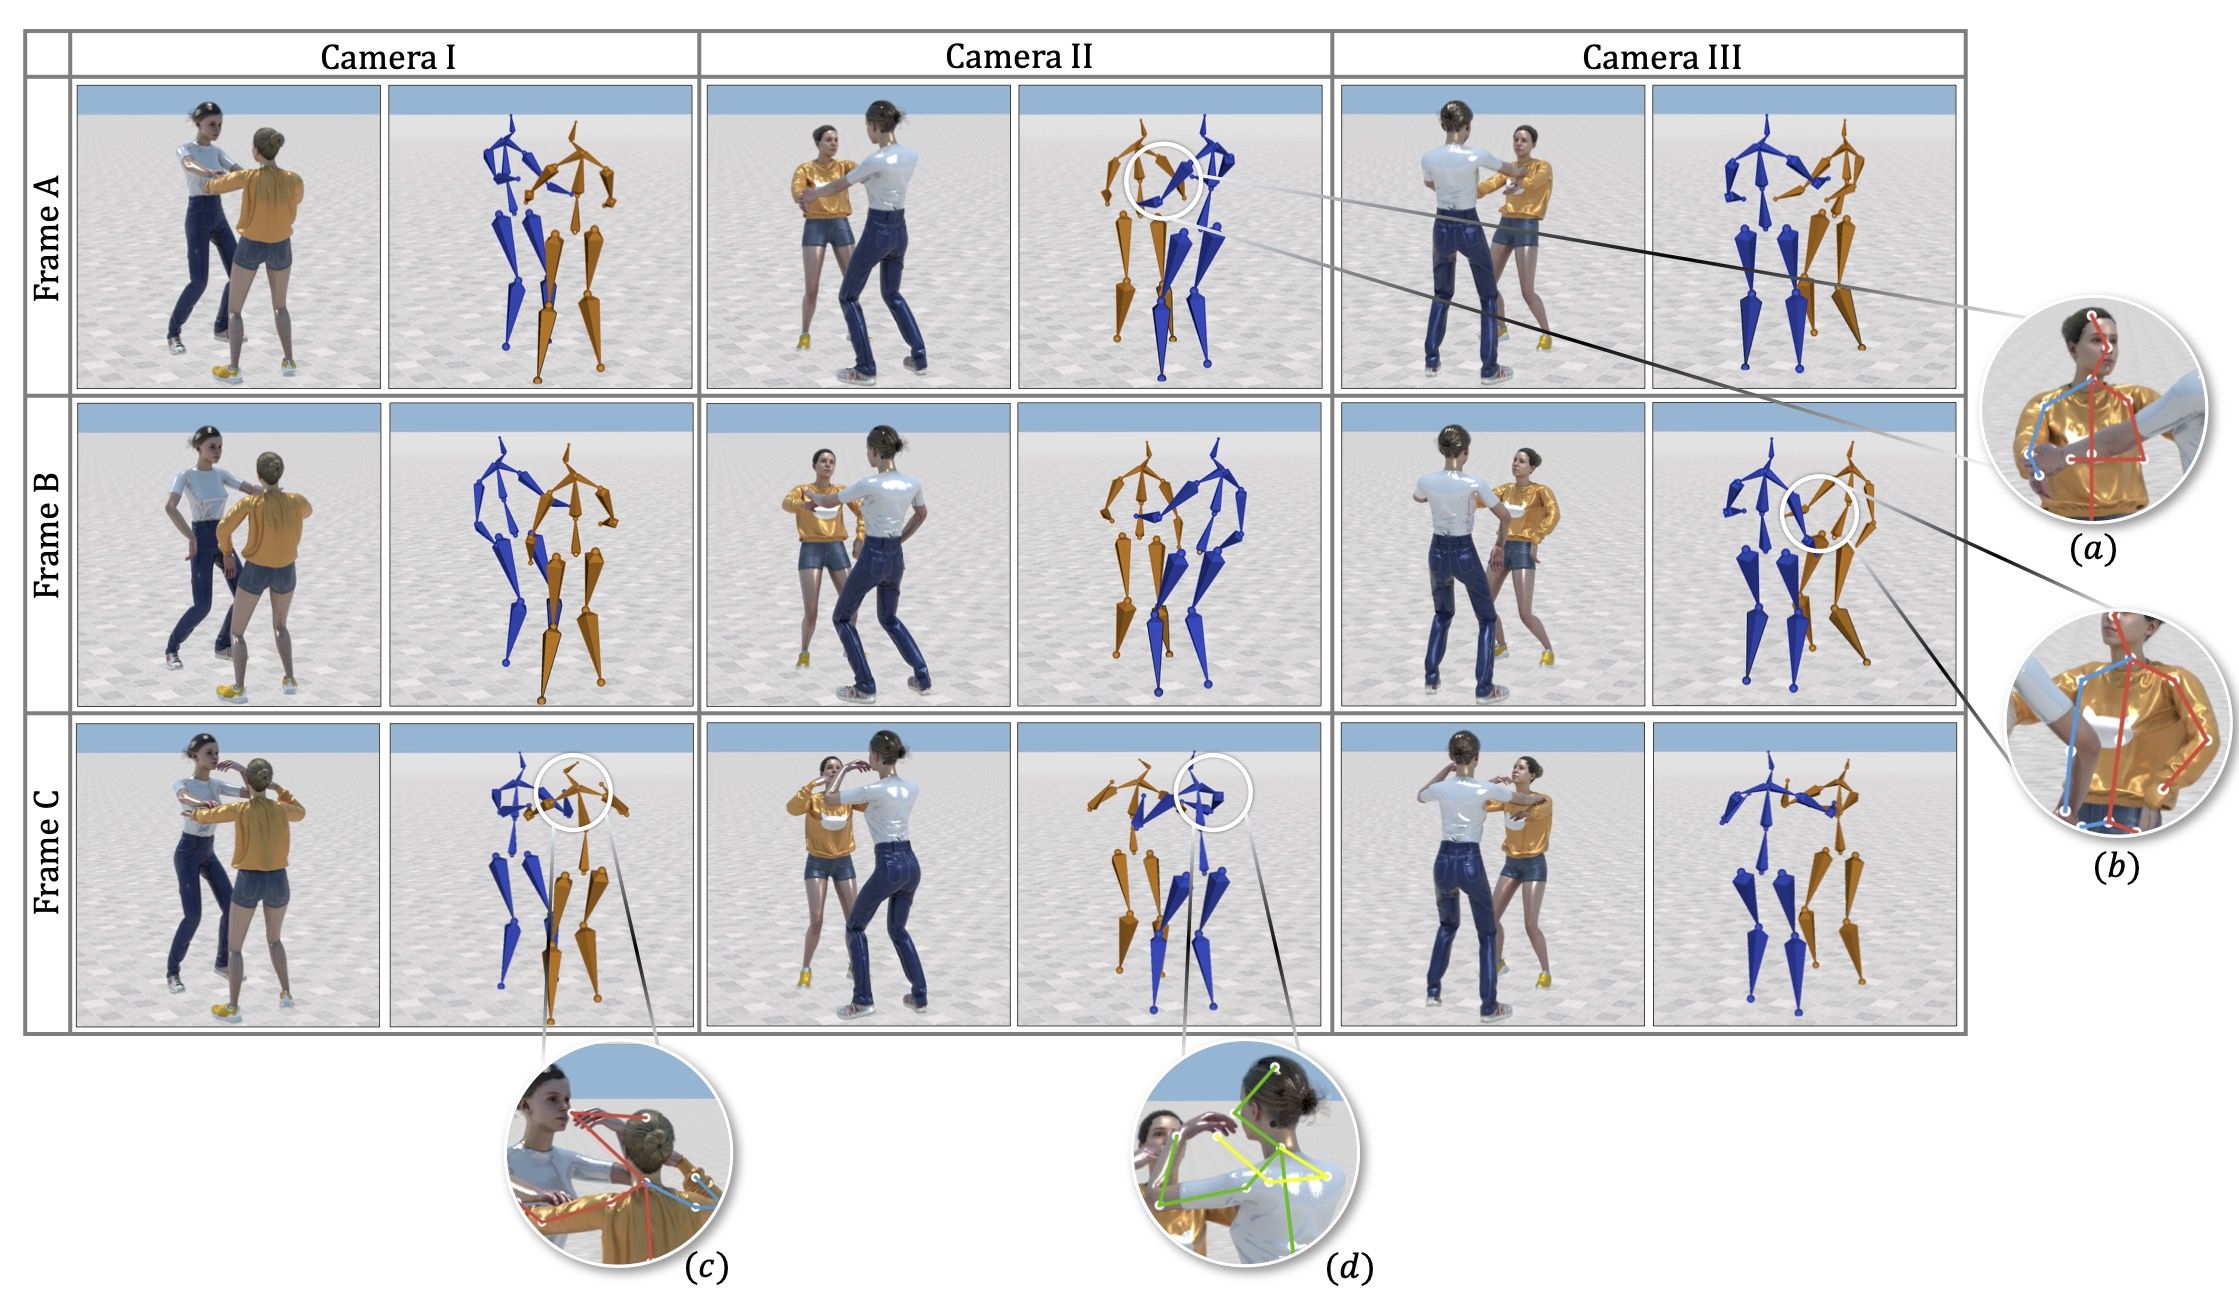
\includegraphics[width=\linewidth]{./images/Macarena_results_with_circles.jpg}
\setlength{\abovecaptionskip}{-10pt plus 3pt minus 2pt}
\setlength{\belowcaptionskip}{-10pt plus 3pt minus 2pt}
\caption{Our results on multi-person synthetic videos, picturing two Macarena dancers. Some of the 2D joints, used as input to our method, are severely inaccurate. However, our method is able to reconstruct correct 3D motion. In the following examples, let \emph{white dancer} and \emph{orange dancer} denote the dancer wearing a white and an orange shirt respectively. Several 2D based skeleton error examples are depicted in the zoomed-in circular insets: 
(a) Wrong pose estimation of the left arm of the orange dancer;
(b) The right arm of the orange dancer is occluded hence detected erroneously; 
(c) The nose tip of the orange dancer is erroneously detected as the nose tip of the white dancer;
(d) Erroneous 2D pose estimation of the white dancer's right hand.}
\label{fig:macarena_results_with_circles}
\end{figure*}